\documentclass[spanish]{article}
\usepackage[utf8]{inputenc}
\usepackage[T1]{fontenc}
\usepackage[spanish]{babel}
\usepackage{graphicx}
\usepackage{wrapfig}
\usepackage{listings}
\usepackage{lipsum}

% ==================================================================================
% Tipos
% ==================================================================================
\usepackage[light,condensed,math]{kurier}


% ==================================================================================
%  Símbolos matemáticos
% ==================================================================================

\usepackage{amsmath}
\usepackage{amsfonts}
\usepackage{amsthm}

\def\N{\ensuremath{\mathbb{N}}}
\def\Z{\ensuremath{\mathbb{Z}}}
\def\Q{\ensuremath{\mathbb{Q}}}
\def\R{\ensuremath{\mathbb{R}}}
\def\C{\ensuremath{\mathbb{C}}}


% ==================================================================================
%  Colores
% ==================================================================================

\usepackage[pdftex]{xcolor}

\definecolor{azulUCA}{cmyk}{1.00, 0.00, 0.00, 0.51}
\definecolor{naranjaUCA}{cmyk}{0.00, 0.51, 1.00, 0.00}
\definecolor{grisUCA}{cmyk}{0.00, 0.00, 0.00, 0.65}
\definecolor{charcoal}{rgb}{0.21, 0.27, 0.31}
\definecolor{darkjose}{HTML}{4a4a4a}
% ==================================================================================
%  Diseño del documento
% ==================================================================================

\usepackage[paperwidth=180mm, paperheight=250mm, top=30mm, bottom=40mm, inner=25mm, outer=20mm]{geometry}

\parskip 5pt
\parindent 0pt

\usepackage[pagestyles]{titlesec}
\titleformat{\chapter}[display]%
{\huge\bfseries}%
{\color{azulUCA}\usefont{T1}{put}{b}{n}\fontsize{70}{80}\selectfont\filleft\thechapter}%
{-60pt}%
{\color{grisUCA}}[\color{grisUCA}]
\usepackage{scrpage2}
\pagestyle{scrheadings}

\clearscrheadfoot                 % deletes header/footer
\pagestyle{scrheadings}           % use following definitions
\cofoot[\pagemark]{\pagemark}     % odd   page, center position
\rohead{\color{grisUCA}{Modelos de la investigación operativa}}
% ==================================================================================
%  Algunos diseños
% ==================================================================================
\usepackage{epigraph}

\newcommand{\citainicial}[1]{
	\raya
	\begin{quotation}
		\color{charcoal}{\textit{#1}}
	\end{quotation}
	\raya
}

\def\raya{
	\par \hbox to
	\linewidth{\hss \vrule width \textwidth height 0.2pt depth 0.5pt}
	\par}

\makeatletter

\usepackage[theorems,breakable]{tcolorbox}

\tcbuselibrary{theorems}


% ==================================================================================
%  Definiciones
% ==================================================================================
\title{\color{azulUCA}{Teoría de colas}\vspace{-6ex}}
\date{}

\usepackage{hyperref}
\hypersetup{
	colorlinks,
	citecolor=black,
	filecolor=black,
	linkcolor=black,
	urlcolor=black
}

\usepackage{titlesec}

\titleformat*{\section}{\LARGE\color{azulUCA}}
\titleformat*{\subsection}{\Large\color{charcoal}}

\begin{document}

% ==================================================================================
% Página inicial
% ==================================================================================
\maketitle
\citainicial{La teoria de colas es útil para administrar correctamente las multitudes, sistemas de entradas y salida, planificación de concesiones y evaluación de flujos de multitudes, venta de entradas, diseño de carreras y planificación, determinar las secuencias de un algoritmo, predecir el rendimiento de un ordenador, de telecomunicaciones, la administración de un hospital (Por ejemplo, el control de las camas de los hospitales), tráfico en los aeropuertos, la industria minera, la capacidad de planificar trenes y autobuses, el análisis del tiempo de la habitat y las estaciones, y más problemas logísticos que puden suponer un problema. \\ \\-  Prof. Dr. G. Keith Still}

\begin{center}
	\href{http://creativecommons.org/licenses/by-sa/3.0/es/}{\includegraphics[width=4em]{cc-by-sa}}
\end{center}

\newpage

\tableofcontents

\newpage

 % ¿Qué es un proceso estocástico?





\section{
	Procesos estocásticos
}

\subsection{Definición} Un \textbf{proceso estocástico }$\lbrace X_t, t \in T \rbrace$ es una colección de variables aleatorias definidas sobre el mismo espacio de probabilidad ($\Omega,S,P$). El conjunto $T$ se llama índice del proceso. Si $T$ es numerable diremos que el proceso estocástico es de tiempo discreto ($T=\lbrace 0,1,2,... \rbrace$) y si es continuo diremos que estamos ante un proceso estocástico de tiempo continuo ($T=\lbrace t, t\geq 0 \rbrace$).

\subsection{Cadena de Markov}\


Sea $\lbrace X_n, n=0,1,2,...\rbrace$ un proceso estocástico de tiempo discreto. Suponemos que en cualquier instante, el proceso toma un número finito o numerable de valores (llamados estados del proceso).
Un proceso estocástico de tiempo discreto es una \textbf{Cadena de Markov}, si para $t$=0,1,2,... y los estados $i_0, i_1,...,i_{n-1},i,j$:

$$
P(X_{n+1}=j|X_n=i, X_{n-1}=i_{n-1},...,X_1=i_1, X_0=i_0)=P(X_{n+1}=j|X_n=i_n)=p_{ij}
$$

donde $X_n=i_n$ representa que en el instante $n$ el proceso se encuentra en el estado $i_n$ y $p_{ij}\geq 0$ la probabilidad de que el proceso pase al estado $j$ cuando se encuentra en el estado $i$.

La matriz de probabilidades de transición en un paso es:


$$P=
\left(
\begin{array}{cccc}
p_{11} & p_{12} & \cdots & p_{1s} \\
p_{21} & p_{22} & \cdots & p_{2s} \\
\vdots & \vdots & & \vdots \\
p_{s1} & p_{s2} & \cdots & p_{ss} \\
\end{array}
\right)
$$
con $ \sum_{j=1}^{s} P(X_{n+1}=j|X_n=i_n)=\sum_{j=1}^{s} p_{ij}=1 $ para $i$=1,2...\\

\textbf{Nota}: Aunque la matriz de probabilidades de transición de un proceso estocástico no tiene por qué ser cuadrada, nos será útil que tenga ésta propiedad para definir probabilidades de transición en la $n$-ésima etapa.\\

\textbf{Ejemplo}:

Sea la matriz de probabilidades en un paso:

$$P=
\left(
\begin{array}{ccc}
1/3 & 1/3 & 1/3 \\
1/3 & 0 & 2/3 \\
1/2 & 1/2 & 0 \\
\end{array}
\right)
$$

Su grafo de estados es:

\begin{figure*}[h]
	\centering
	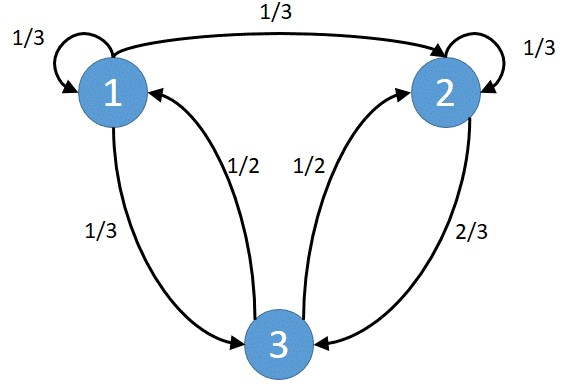
\includegraphics[width=0.4\textwidth]{grafo1}
	\label{grf1}
\end{figure*}



\subsection{Probabilidades de transición en la $\textbf{\textsl{n}}$-ésima etapa}

Supongamos que una cadena de Markov, en el instante $m$ está en el estado $i$, ¿Cuál es la probabilidad de estar en el estado $j$ después de n periodos? Esta probabilidad es independiente de $m$, así que la podemos escribir como:

$$
P(X_{m+n}=j|X_m)=P(X_n=j|X_0=i)=p_{ij}^n
$$

donde $p_{ij}^n$ se llama probabilidad del $n$-ésimo paso de transición del estado $i$ al $j$ y son los $ij$-ésimos elementos de $P^n$, donde $P$ es la matriz de probabilidades en un paso de nuestra cadena de Markov.\\


\textbf{Ejemplo}:\\ 

Sea P la matriz de probabilidades de transición en un paso del ejemplo anterior. Calcula todas las probabilidades de transición en dos pasos.


$$P^2=
\left(
\begin{array}{ccc}
1/3 & 1/3 & 1/3 \\
1/3 & 0 & 2/3 \\
1/2 & 1/2 & 0 \\
\end{array}
\right)
\left(
\begin{array}{ccc}
1/3 & 1/3 & 1/3 \\
1/3 & 0 & 2/3 \\
1/2 & 1/2 & 0 \\
\end{array}
\right)
=
\left(
\begin{array}{ccc}
21/54 & 15/54 & 18/54 \\
24/54 & 24/54 & 6/54 \\
18/54 & 9/54 & 27/54 \\
\end{array}
\right)
=
\left(
\begin{array}{cccc}
p_{11}^2 & p_{12}^2 & p_{13}^2 \\
p_{21}^2 & p_{22}^2 & p_{23}^2 \\
p_{31}^2 & p_{32}^2 & p_{33}^2 \\
\end{array}
\right)
$$

$\linebreak$

Se puede observar que cuando $n$ es suficientemente grande las probabilidades de transición del estado $i$ al estado $j$ en $n$ pasos se estabilizan, esto quiere decir, 

$$
p_{ij}^{n+1}\cong p_{ij}^n
$$
cuando $n$ es grande.

Definimos el vector $\pi=[\pi_1 \, \pi_2 \, \cdots \, \pi_s]$ como el \textbf{vector de distribución de estado estable}, donde, para cada $j$=1,2,..,s se tiene que:

$$
\lim_{n \to \infty} p_{ij}^n = \pi_j 
$$

para todo $i$=1,2,..,s.

% Proceso de nacimiento muerte.


\section{Procesos de nacimiento y muerte}

Para analizar este tipo de procesos definimos el número de personas presentes en el sistema en el tiempo $t$ como el estado del sistema en ese tiempo $t$. Consideramos $p_{ij}^n$ la probabilidad de que, habiendo $i$ personas en el sistema, después de $n$ pasos halla $j$ personas. Hemos visto anteriormente que cuando $n$ es suficientemente grande esas probabilidades se estabilizan en $\pi_j$. Diremos que $p_{ij}^n$ tiene un \textbf{comportamiento transitorio} si $p_{ij}^n$ aún no ha alcanzado el estado estable. Por ahora, supondremos que el estado estable ya se alcanzó y trabajaremos con $\pi_j$.

\subsection{Leyes de movimiento}

Sea $\lbrace X(t), t\geq 0 \rbrace$ el proceso de tiempo continuo que indica el número de personas en el sistema en el tiempo $t$ y $S=\lbrace 0,1,2,.,j,..\rbrace$ el espacio de estados. Supongamos que para cierto $t$, $X(t)=j$. Los procesos de nacimiento-muerte se rigen por tres leyes básicas:

\begin{enumerate}
	
	\item $P$(1 nacimiento entre $(t, t+h)$)=$\lambda_j h +o(h)$.\\
	El estado se incrementa en 1, esto es, $X(t+h)=j+1$.
	$\lambda_j$ es la tasa de nacimiento en el estado $j$ (equivaldría a una llegada).
	
	\item $P$(1 muerte entre $(t, t+h)$)=$\mu_j h +o(h)$.\\
	El estado se disminuye en 1, esto es, $X(t+h)=j-1$.
	$\mu_j$ es la tasa de muerte en el estado $j$ (equivaldría a una salida).
	
	\item Los nacimientos y muertes son independientes.
	
	
\end{enumerate} 

\begin{figure}[h]
	\centering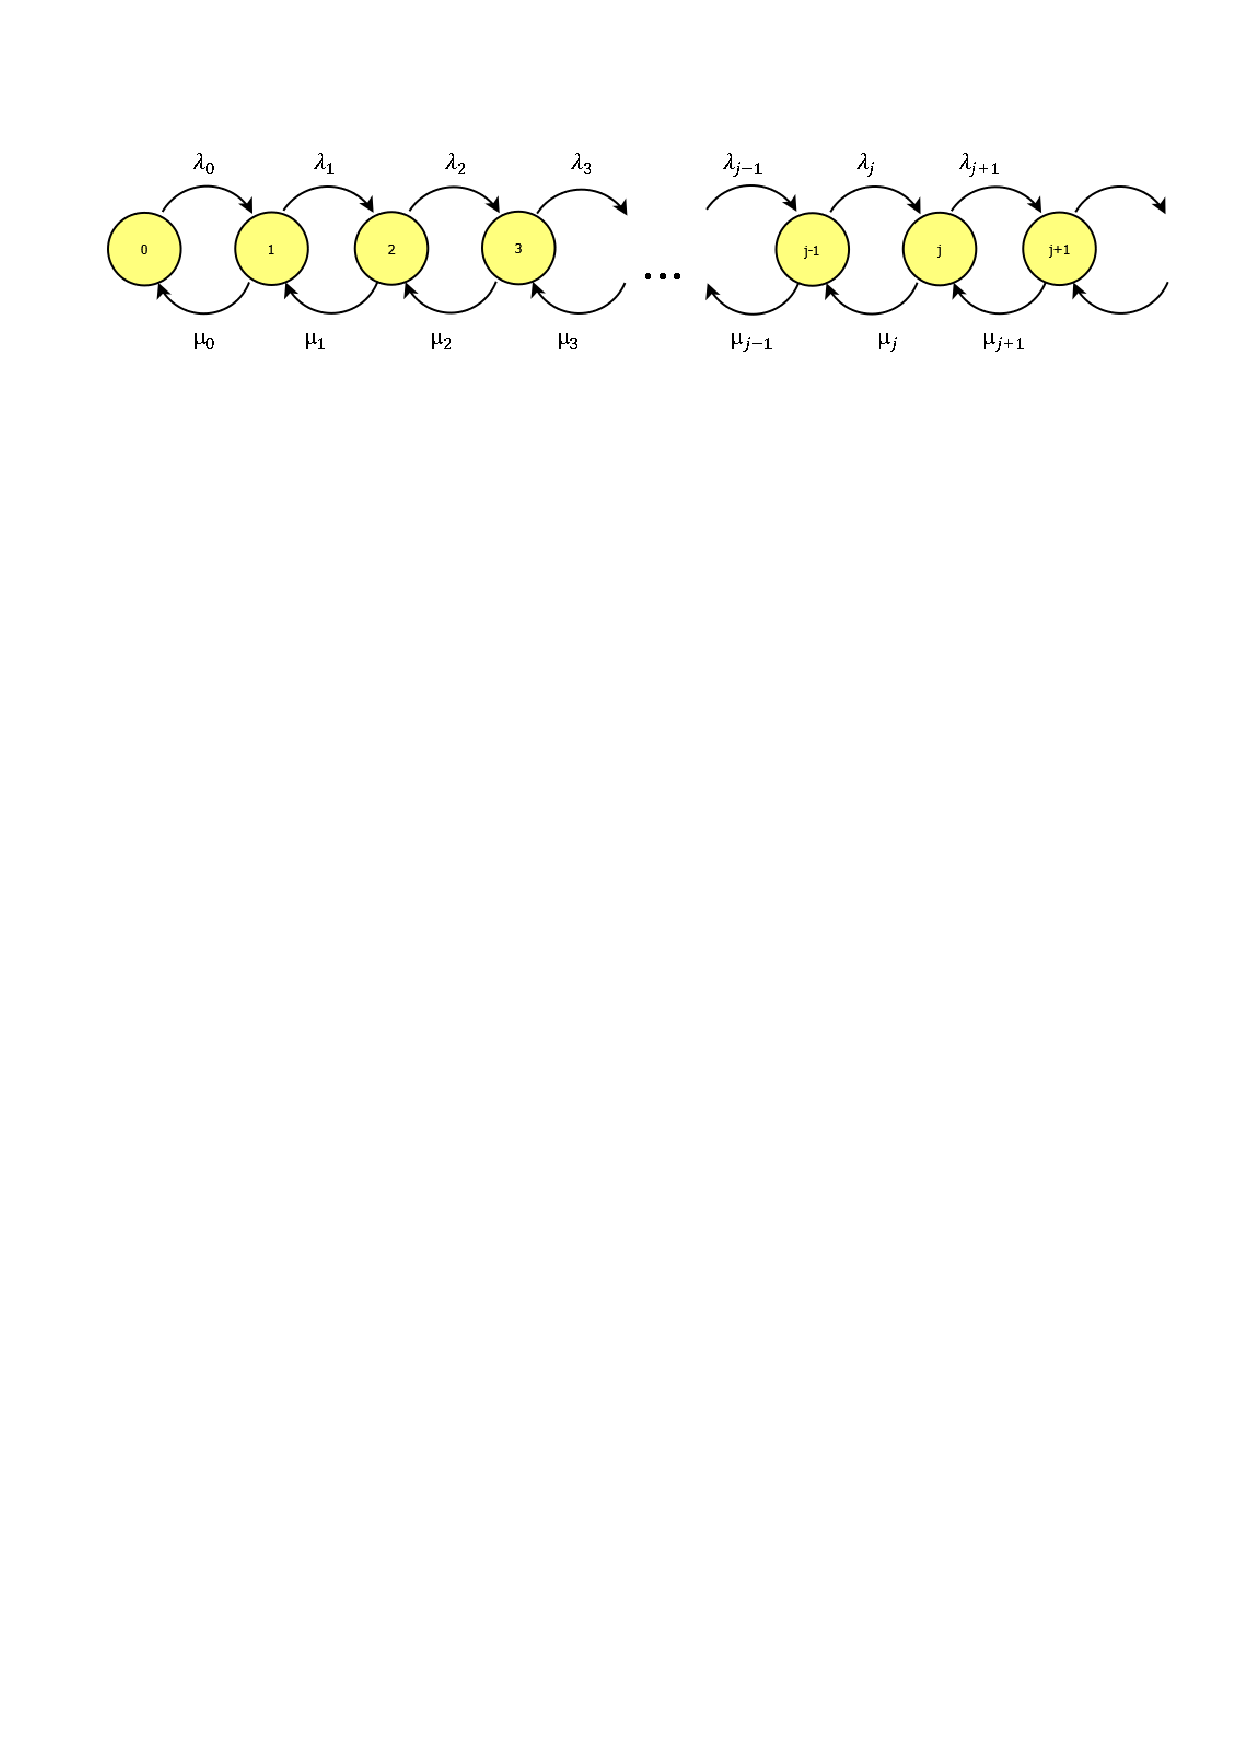
\includegraphics[trim = 10mm 220mm 10mm 25mm, clip,width=0.9\linewidth]{diagramatasa}
	\caption{Diagrama de tasas}
\end{figure}

Consideremos que tanto los nacimientos como las muertes siguen distribuciones exponenciales de parámetros $\lambda$ y $\mu $ respectivamente. \\
Por la carencia de memoria de la distribución exponencial, la probabilidad de que un nacimiento ocurra durante $(t,t+h)$ es de:

$$
\int_{0}^{h}  \lambda \, e^{-\lambda t} \, dt = 1-e^{-\lambda h}=1-(1-\lambda h + o(h))=\lambda h + o(h)
$$

Del mismo modo, la probabilidad de que ocurra una muerte durante $(t,t+h)$ es de:

$$
\int_{0}^{h}  \mu \, e^{-\mu t} \, dt = 1-e^{-\mu h}=1-(1-\mu h + o(h))=\mu h + o(h)
$$ 

Es posible desarrollar un modelo modificado de nacimiento-muerte con los tiempos de llegada y servicio siguiendo distribuciones Erlang.

\subsection{Cálculo de $\pi_j$}

Para determinar las $\pi_j$ relacionamos $p_{ij}(t)$ con $p_{ij}(t+h)$ para $h$ pequeña. 

Es fácil ver que

\begin{equation*}
\begin{split}
p_{ij}(t+h)= p_{i,j-1}(t)P(\textrm{1 nacimiento en } (t,t+h))+\\
+ p_{i,j+1}(t)P(\textrm{1 muerte en }(t,t+h))+\\
+ p_{ij}(t)P(\textrm{ningún nacimiento ni muerte en }(t,t+h))
\end{split}
\end{equation*}

Esto es


\begin{equation}
\begin{split}
p_{ij}(t+h)= p_{i,j-1}(t)(\lambda_{j-1}h + o(h))+\\
+ p_{i,j+1}(t)(\mu_{j+1}h + o(h))+\\
+ p_{ij}(t)(1-\lambda_{j}h - \mu_{j}h + o(h) )
\end{split}
\end{equation}



Reagrupando:

\begin{equation*}
p_{ij}(t+h) = p_{ij}(t) + h(\lambda_{j-1} p_{i,j-1}(t) + \mu_{j+1}  p_{i,j+1}(t) - \lambda_j  p_{ij} - \mu_{j} p_{ij}(t) + o(h))
\end{equation*}



Restando a ambos lados de la igualdad $p_{ij}(t)$ y dividiendo entre $h$ tenemos:


\begin{equation*}
\frac{p_{ij}(t+h)-p_{ij}(t)}{h}=\lambda_{j-1} p_{i,j-1}(t) + \mu_{j+1}  p_{i,j+1}(t) - \lambda_j  p_{ij}(t) - \mu_{j} p_{ij}(t) + o(h)
\end{equation*}

Tomando límite de $h$ tendiendo a 0 nos queda:


\begin{equation*}
p_{ij}'(t)= \lambda_{j-1} p_{i,j-1}(t) + \mu_{j+1}  p_{i,j+1}(t) - \lambda_j  p_{ij}(t) - \mu_{j} p_{ij}(t)
\end{equation*}

Para $t$ grande y cualquier estado inicial $i$, $p_{ij}(t)=\pi_{j}$ constante. Por lo tanto, $p_{ij}(t)'=0$. Sustituyendo todos las probabilidades de estado estable en la ecuación, se tiene:

\begin{equation*}
\lambda_{j-1} \pi_{j-1} + \mu_{j+1}  \pi{j+1} - \lambda_j  \pi_{j} - \mu_{j} \pi_{j}=0
\end{equation*}

\begin{equation}
\lambda_{j-1} \pi_{j-1} + \mu_{j+1}  \pi_{j+1} = \pi_j(\lambda_j + \mu_j) \qquad (j= 1,2,...) \label{eq1}
\end{equation}


Para $j=0$, tenemos:

\begin{equation}
\mu_1 \pi_1 = \pi_0 \lambda_0
\label{eq2}
\end{equation}

Las ecuaciones ($\ref{eq1}$) y ($\ref{eq2}$) se llaman \textbf{ecuaciones de balance de flujo} para un proceso de nacimiento-muerte.\\

\textbf{Solución de las ecuaciones de balance de flujo en un proceso de nacimiento-muerte:}\\

Primero, expresamos todas las $\pi_j$ en función del término $\pi_0$.\\

De (\ref{eq2}) obtenemos

\begin{equation}
\pi_1=\frac{\pi_0 \lambda_0}{\mu_1}
\label{eq3}
\end{equation}

Al sustituir (\ref{eq3}) en (\ref{eq1}) para $j=1$ y despejando $\pi_2$ tenemos

\begin{equation}
\pi_2=\frac{\pi_0(\lambda_0 \lambda_1)}{\mu_1 \mu_2}
\label{eq4}
\end{equation}

Procediendo análogamente para $j=3,4,..$ se tiene que

\begin{equation}
\pi_j=\pi_0 c_j
\label{eq5}
\end{equation}

donde $c_j=\dfrac{\lambda_0 \lambda_1 \cdots \lambda_{j-1}}{\mu_1 \mu_2 \cdots \mu_j}$.\\

Como debemos estar en algún estado para cualquier tiempo $t$:

\begin{equation}
\sum_{j=0}^{\infty}\pi_j=1 
\label{eq6}
\end{equation}

Sustituyendo ($\ref{eq5}$) en (7) se llega a

\begin{equation*}
\pi_0 \left( 1+\sum_{j=1}^{\infty} c_j \right) = 1 
\end{equation*}

Despejando $\pi_0$, si la serie es convergente:

\begin{equation}
\pi_0=\dfrac{1}{1+\sum_{j=1}^{\infty} c_j}
\label{eq6}
\end{equation}

Por lo tanto, una vez que calculemos $\pi_0$ utilizando $(6)$ podremos calcular cualquier $\pi_j$ mientras estemos en estado de equilibrio. \\
Se puede demostrar que si:
$$
\sum_{j=1}^{\infty} c_j = \infty $$
Entonces el sistema no existe una distribución de estado estable.

% Introducción al sistema  de líneas de espera


\section{Introducción al sistema de líneas de espera}
\subsection{Procesos de llegadas}
En este contexto, definimos las llegadas como los clientes que llegan. Para este tipo de problemas solemos asumir que, en un instante dado, no puede haber más de una llegada. Cuando es posible que llegue más de un cliente en un mismo instante de tiempo, decimos que permitimos llegadas a granel (bulk arrivals).\\
Normalmente, un proceso de llegadas no se ve afectado por el número de clientes que presenta el sistema.\\
Hay dos situciaciones comunes en las cuales el proceso de llegada podría depender del número de clientes.
\begin{itemize}
	\item \textbf{Modelos de origen finito:} Ocurre cuando las llegadas están sacadas de una población pequeña.
	\item \textbf{Razón:} Ocurre cuando la razón a la cual llegan los clientes a cierta instalación disminuye cuando ésta se llena. Si un cliente llega, pero se retira del sistema, se dice que el cliente ha renunciado.
\end{itemize} 

Si el número de clientes presente no afecta al proceso de llegadas, entonces se le describe mediante la especificación de la distribución de probabilidad que rige el tiempo entre llegadas sucesivas.

\subsection{Procesos de salida}
Para describir el proceso de salida (con frecuencia se le llama proceso de servicio) de un sistema de líneas de espera, se especifica una distribución de probabilidad, \textbf{distribución de tiempo de servicio}, que rige el tiempo de servicio a un cliente. En la mayoría de casos, esta distribución del tiempo de servicio es independiente de la cantidad de clientes presentes. (De aquí se infiere que el servidor, o canal, no trabaja más rápido cuando hay más clientes presentes).
\\ Existen dos tipos de servidores:
\begin{itemize}
	\item \textbf{Servidores en paralelo:} Los servidores están en paralelo si todos ofrecen el mismo tipo de servicio y un cliente sólo requiere pasar por un servidor para completar el servicio.
	\item\textbf{Servidores en serie:}Los servidores están en serie cuando un cliente debe pasar por varios servidores antes de terminar el servicio.
\end{itemize}
\subsection{Disciplina de las líneas de espera}
Para describir por completo un sistema de líneas de espera , se debe describir también la disciplina de las líneas de espera y el modo en el cual los clientes forman las líneas de espera. Esta disciplina explica el método usado para determinar el orden en el que se atiende a los clientes.
\\ Existen varios tipos de disciplina:
\begin{itemize}
	\item \textbf{Disciplina FCFS:}(al primero que llega se le atiende primero). Se atiende a los clientes según el orden en que llegan.
	\item\textbf{Disciplina LCFS:}(El último en llegar es el primero en salir). Las llegadas más recientes son los primeros clientes en entrar al servicio.
	\item\textbf{Disciplina SIRO:} (Servicio en orden aleatorio). El siguiente cliente en pasar al servidor es elegido en forma aleatoria de entre los clientes que están esperando atención.
	\item\textbf{Disciplina de prioridad en las colas:} Una disciplina en prioridad clasifica cada llegada en una categoría. Cada categoría recibe luego un nivel de prioridad, y dentro de cada nivel de prioridad, los clientes entran en el servicio siguiendo FCFS.
	
\end{itemize}

\subsection{Notación Kendall-Lee}
La notación que se estudia en esta sección sirve para caracterizar un sistema de líneas de espera en el cual todas las llegadas esperan en una sola cola hasta que está libre uno de lo\textit{s} servidores paralelos idénticos. Luego el primer cliente en la cola  entra al servicio, y así sucesivamente (véase figura). Por ejemplo, si el cliente en el servidor 3 es el siguiente para completar servicio, entonces (si se supone una disciplina FCFS) el primer cliente en la cola entraría al servidor 3. El cliente siguiente en la cola entraría al servicio después de finalizar el servicio siguiente, etc.
\\
Kendall (1951) diseñó la notación siguiente para representar dicho sistema de líneas de espera. Cada sistema de líneas de espera se describe mediante seis características:
1/2/3/4/5/6

La primera característica especifica la naturaleza del proceso de llegada. Se utilizan las abreviaturas estándar siguientes:
\begin{itemize}
	\item M=Los tiempos entre llegadas son variables aleatorias independientes e idénticamente distribuidas (iid) cuya distribución es exponencial.
	\item D = Los tiempos entre llegadas son iid y deterministas.
	\item $E_k$ = Los tiempos entre llegadas son Erlangs iid con parámetro de forma k.
	\item GI = Los tiempos entre llegadas son iid y están regidos por alguna distribución general.
\end{itemize}
La segunda característica especifica la naturaleza de los tiempos de servicio:
\begin{itemize}
	\item M = Los tiempos de servicio son iid y están distribuidos exponencialmente.
	\item D = Los tiempos de servicio son iid y deterministas.
	\item $E_k$ = Los tiempos de servicio son Erlangs iid con un parámetro de forma k.
	\item G= Los tiempos de servicio son iid y están regidos por alguna distribución general.
\end{itemize}
La tercera característica es la cantidad de servidores en paralelo. 
\\ La cuarta característica es la disciplina de líneas de espera:
\begin{itemize}
	\item FCFS = El primero en llegar, primero en ser atendido.
	\item LCFS = El último en entrar, primero en salir.
	\item SIRO = Servicio en orden aleatorio.
	\item GD = Disciplina general de líneas de espera.
\end{itemize}
La quinta característica específica el número máximo admisible de clientes en el sistema (incluidos los clientes que están esperando y los que están en servicio). 
\\ La sexta característica da el tamaño de la población de donde se extraen los clientes. A menos que la cantidad de clientes potenciales sea del mismo orden de magnitud que el número de servidores, la población se considera infinito. En muchos modelos importantes 4/5/6 es GD/$\infty$/$\infty$. Si así sucede, entonces 4/5/6 se omite, a menudo.
\\
Como ejemplo de esta notación, M/$E_2$/8/FCFS/10/$\infty$ podría representar una clínica con ocho médicos, tiempos entre llegadas exponenciales, tiempos de servicio de Erlangs de dos fases, una disciplina de líneas de espera FCFS y una capacidad total de 10 pacientes. \\
Si no se especifica, tanto la capacidad del sistema como la población serán $\infty$ y la política de llegada será $FCFS$.


% Modelos de colas
	\section{Fórmulas de Little}
	Hay ciertos datos que nos pueden resultar muy interesantes de obtener, como el n\'umero medio de personas en el sistema o el tiempo medio que un cliente pasa en \'el. Definimos los siguientes t\'erminos:
	\begin{itemize}
		\item $\lambda$ = ratio de entrada de clientes por unidad de tiempo
		\item$L$ = n\'umero medio de clientes en el sistema
		\item$L_q$ = n\'umero medio de clientes en la cola
		\item$L_s$ = n\'umero medio de clientes siendo servidos
		\item$W$ = tiempo medio que un cliente pasa en el sistema
		\item$W_q$ = tiempo medio que un cliente pasa en la cola
		\item$W_s$ = tiempo medio que un cliente tarda en ser servido
	\end{itemize}
\hspace{0.5cm}	En estas definiciones, siempre asumimos que estamos en el estado de equilibrio. Para la mayor\'ia de colas, podemos escribir las f\'ormulas de Little como en el siguiente teorema.
	\subsection{Teorema}
	Para cualquier sistema de colas en el que exista el estado estable, se tienen las siguientes relaciones:
	\begin{itemize}
		\item $L=\lambda W$
		\item$L_q=\lambda W_q$
		\item$L_s=\lambda W_s$
	\end{itemize}
\hspace{0.5cm}	Vamos a dar una prueba intuitiva, debido a la gran dificultad de la prueba anal\'itica. \\
\hspace{0.5cm}Consideramos un sistema de colas con pol\'itica FCFS. Supongamos una llegada arbitraria. Cuando este cliente abandone el sistema, habr\'a de media en el sistema $L$ clientes. Por otro lado, cuando este cliente se haya, las personas que queden en el sistema ser\'an aquellas que han llegado en el tiempo que el cliente ha pasado en el sistema, $W$. Como el ratio de entrada es $\lambda$, tenemos que $L=\lambda W$.\\
\hspace{0.5cm}	Es interesante saber que la prueba anal\'itica es independiente de la pol\'itica de servicio, el n\'umero de servicios, la distribuci\'on del tiempo de llegada y del tiempo de servicio, por lo que las f\'ormulas de Little nos ser\'an v\'alidas en cualquier sistema de colas en el que se pueda alcanzar el estado de equilibrio.

\section{M/M/1}
En este modelo, el tiempo entre llegada sigue una distribuci\'on exponencial (suponemos que $\lambda$ es el ratio de llegada por unidad de tiempo) y el servidor tiene tiempos de servicio exponenciales ( suponemos que el ratio de tiempo de servicio es $\mu$ ). Como ya hemos demostrado, este modelo puede ser representado como un proceso de nacimiento-muerte con los siguientes par\'ametros:
	$$\begin{array}{cc}
	\lambda_j=\lambda & (j=0,1,...)\\
	\mu_0=0 &  \\
	\mu_j=\mu &  (j=1,2,...)\\
	\end{array}$$
	
Con estos par\'ametros y sabiendo que $\pi_j=\pi_0 c_j$ tenemos que:
	\begin{center}
		$\pi_1=\pi_0\rho, \qquad \pi_2=\pi_0\rho^2, \qquad...,\qquad\pi_j=\pi_0\rho^j$
	 
	\end{center}
\hspace{0.5cm}Donde $\rho=\frac{\lambda}{\mu}$, a lo que llamaremos intensidad de tr\'afico. Como la suma de todos los estados es $1$ llegamos a:
	\begin{center}
		$$\sum_{j=0}^{\infty}\pi_j=\pi_0(1+ \rho +\rho^2+\rho^3+...)=1$$
	\end{center}
\hspace{0.5cm}Vamos a asumir que $0\leq rho<1$. Vamos a calcular $S=1+ \rho +\rho^2+\rho^3+...$. Para ello multiplicamos $S$ por $\rho$, $S\rho=\rho+\rho^2+\rho^3+...$ y hacemos $S-\rho S=1$, de donde $S=\frac{1}{1-\rho}$.\\
\hspace{0.5cm}Sustituyendo en por el valor obtenido de $S$
	\begin{center}
		$\pi_0=1-\rho$
	\end{center}
\hspace{0.5cm}Y sustituyendo en la expresi\'on que tenemos para $\pi_j$ finalmente llegamos al resultado
	\begin{center}
		$\pi_j=\rho^j(1-\rho)$
	\end{center}
\hspace{0.5cm}Hemos asumido que $0\leq\rho<1$ para hallar la expresi\'on de $\pi_j$. Si $\rho>1$ entonces se tiene que $\lambda>\mu$, y por lo tanto el sistema no alcanzar\'ia el estado de equilibrio, ya que el ritmo de entrada de clientes ser\'ia mayor que el de salida, y por lo tanto la cantidad de gente en el sistema se disparar\'ia.\\
\hspace{0.5cm}Si $\rho=1$ no se puede ver de forma tan clara que no se alcanza el estado de equilibrio, pero tendr\'iamos que $S=1+1+1+1+...$ lo cual diverge.
	\subsection{C\'alculo de $L$}
	A partir de ahora siempre asumimos que $\rho<1$, y que hemos alcanzado el estado de equilibrio. Como $\pi_j$ indica la probabilidad de que haya $j$ individuos en el sistema, el n\'umero medio de personas en el sistema vendr\'a dado por
		\begin{center}
			$$L=\sum_{j=0}^{\infty}j\pi_j=\sum_{j=0}^{\infty}j\rho^j(1-\rho)=(1-\rho)\sum_{j=0}^{\infty} j \rho^j$$
		\end{center}  
	\hspace{0.5cm}Sea $S_2=\displaystyle \sum_{j=0}^{\infty}j\rho^j=\rho+2\rho^2+3\rho^3...$\\
	\hspace{0.5cm}Al igual que antes, hacemos $\rho S_2$ y restando: $$S_2 -\rho S_2=\rho+\rho^2+\rho^3...=\frac{\rho}{1-\rho}$$
	Despejando, tenemos que $S_2=\displaystyle\frac{\rho}{(1-\rho)^2}$ y por lo tanto
		\begin{equation}
			L=(1-\rho)\frac{\rho}{(1-\rho)^2}=\frac{\rho}{1-\rho}=\frac{\lambda}{\mu-\lambda}
		\end{equation}
	
	\subsection{C\'alculo de $L_q$ y $L_s$}
	En el modelo $M/M/1$ siempre habr\'a una persona siendo servida, excepto si no hay ninguna persona en el sistema. Por lo tanto, el n\'umero medio de personas siendo servidas $L_s$, ser\'a
		\begin{center}
			$$L_s=0\pi_0+1(\pi_1+\pi_2+...)=1-\pi_0=1-(1-\rho)=\rho$$
		\end{center}
\hspace{0.5cm}	Adem\'as, todos los clientes que est\'en en el sistema o bien est\'an en la cola o bien est\'an siendo servidos, es decir, $L=L_q+L_s$. Por lo tanto
		\begin{center}
			$$L_q=L-L_s=\frac{\rho^2}{1-\rho}$$
		\end{center}
	
	\subsection{C\'alculo de los tiempos de espera}
	Usando las f\'ormulas de Little podemos calcular f\'acilmente $W,W_q$ y $W_s$
		\begin{itemize}
			\item $W=\displaystyle\frac{L}{\lambda}=\frac{1}{\mu-\lambda}$
			\item $W_q=\displaystyle\frac{L_q}{\lambda}=\frac{\lambda}{\mu(\mu-\lambda)}$
			\item$W_s=\displaystyle\frac{L_s}{\lambda}=\frac{1}{\mu}$
		\end{itemize}
	\hspace{0.5cm}Al igual que con la cantidad media de individuos, podr\'iamos haber usado que un cliente pasa su tiempo en el sistema o esperando en la cola o siendo servido, es decir, $W=W_q+W_s$. \\
	\hspace{0.5cm}Como observaci\'on, el valor de $W_s$ lo pod\'iamos deducir desde un principio, pues al ser el tiempo del servidor exponencial de par\'ametro $\mu$, su esperanza es $\displaystyle \frac{1}{\mu}$.
	
\section{M/M/1/c}
		En este modelo, a diferencia del $M/M/1$ el sistema tiene una capacidad $c$. Se comportará igual a la $M/M/1$, excepto cuando haya $c$ personas en el sistema, momento en el cual todas las nuevas llegadas no podrán entrar en el sistema, y diremos que estas se han perdido. Suponiendo tiempos entre llegada exponenciales de ratio $\lambda$ y tiempos de servicio exponenciales de ratio $\mu$, podemos modelar esta cola como un proceso de nacimiento-muerte con los siguientes par\'ametros:
		$$\begin{array}{cc}
		\lambda_j=\lambda & (j=0,1,...,c-1)\\
		\lambda_c=0 & \\
		\mu_0=0 &  \\
		\mu_j=\mu &  (j=1,2,...,c)\\
		\end{array}$$
		\hspace{0.5cm} Como $\lambda_c=0$, la probabilidad de llegar al estado $c+1$ es $0$. Por lo tanto, las ecuaciones de balance ser\'ian:
			$$\begin{array}{cc}
		\pi_0=\displaystyle\frac{1-\rho}{1-\rho^{c+1}} & \\
		\pi_j=\rho^j\pi_0 & (j=1,2,...,c)\\
		\pi_j=0 & (j=c+1,c+2,...)\\
		\end{array}$$
		\subsection{C\'alculo de $L$} A diferencia del modelo $M/M/1$, en el $M/M/1/c$ es posible que $\rho\geq1$, ya que en este caso la cantidad de clientes no se disparar\'ia ya que cuando se llegase a $c$ clientes nadie m\'as podr\'ia entrar al sistema. Para el c\'alculo de $L$ vamos a diferenciar dos posibles casos para $\rho$
		\begin{itemize}
			\item  Si $\rho=1$ tenemos que 
			$$\begin{array}{cc}
				\pi_j=\frac{1}{c+1} & (j=0,1,...,c)\\
				L=\displaystyle\sum_{k=0}^{c}k\pi_k=\frac{1}{c+1}\sum_{k=0}^{c}k=\frac{c}{2}& \\
				\end{array}$$
		
			\item Si $\rho\neq1$

					$$L=\sum_{k=0}^{c}k\frac{\rho^k (1-\rho)}{1-\rho^{c+1}}=\frac{1}{1-\rho^{c+1}}\sum_{k=0}^{c}k\rho^k (1-\rho)=\frac{1}{1-\rho^{c+1}}(\underbrace{\sum_{k=0}^{\infty}k\rho^k(1-\rho)}_{\displaystyle\frac{\rho}{1-\rho^{c+1}}}-\sum_{k=c+1}^{\infty}k\rho^k(1-\rho))$$
					$$\sum_{k=c+1}^{\infty}k\rho^k(1-\rho)=\sum_{k=c+1}^{\infty}[k-(c+1)+(c+1)]\rho^k(1-\rho)=$$
					$$\sum_{k=c+1}^{\infty}[k-(c+1)]\rho^k(1-\rho)+\sum_{k=c+1}^{\infty}(c+1)\rho^k(1-\rho)=$$
					$$\rho^{c+1}\sum_{m=0}^{\infty}m\rho^m(1-\rho)+(c+1)\rho^{c+1}\sum_{m=0}^{\infty}\rho^m(1-\rho)=\rho^{c+1}\frac{\rho}{1-\rho}+(c+1)\rho^{c+1}$$

				Entonces acabamos diciendo que 
				\begin{center}
					$L=\frac{1}{1-\rho^{c+1}}((1-\rho^{c+1})\frac{\rho}{1-\rho}-(c+1)\rho^{c+1})=\frac{\rho}{1-\rho}-\frac{(c+1)\rho^{c+1}}{1-\rho^{c+1}}$
				\end{center}
			\subsection{C\'alculo de $L_q$ y $L_s$}
			\hspace{0.5cm} Al solo haber un \'unico servidor, el c\'alculo de $L_s$ es igual que en el modelo $M/M/1$
				$$L_s=1-\pi_0$$
			Una vez tenemos $L$ y $L_s$, es muy f\'acil obtener $L_q$
				$$L_q=L-L_s=L-1+\pi_0$$
			\subsection{C\'alculo de $W$,$W_q$ y $W_s$}
			\hspace{0.5cm}En este modelo, tenemos que $\lambda$ es el n\'umero medio de personas que llegan al sistema por unidad de tiempo. Pero al tener una capacidad finita, no todas las personas que llegan entran, pues si hay $c$ personas, el siguiente cliente en "llegar" $~$ no podr\'a entrar. Por lo tanto, la cantidad media de clientes que realmente entrar\'a en el sistema ser\'a $\lambda-\lambda\pi_c=\lambda(1-\pi_c)$. Por lo tanto, usando las f\'ormulas de Little:
			\begin{itemize}
				\item $\displaystyle W=\frac{L}{\lambda(1-\pi_0}$
				\item $\displaystyle W_q=\frac{L_q}{\lambda(1-\pi_c)}$
			\end{itemize}
	\hspace{0.5cm}	Como el tiempo que tarda cada servidor es una exponencial de ratio $\mu$, tenemos que al igual que en el modelo $M/M/1$, $W_s=\frac{1}{\mu}$.
		\end{itemize}
		
		
		\begin{figure}[h]
			\centering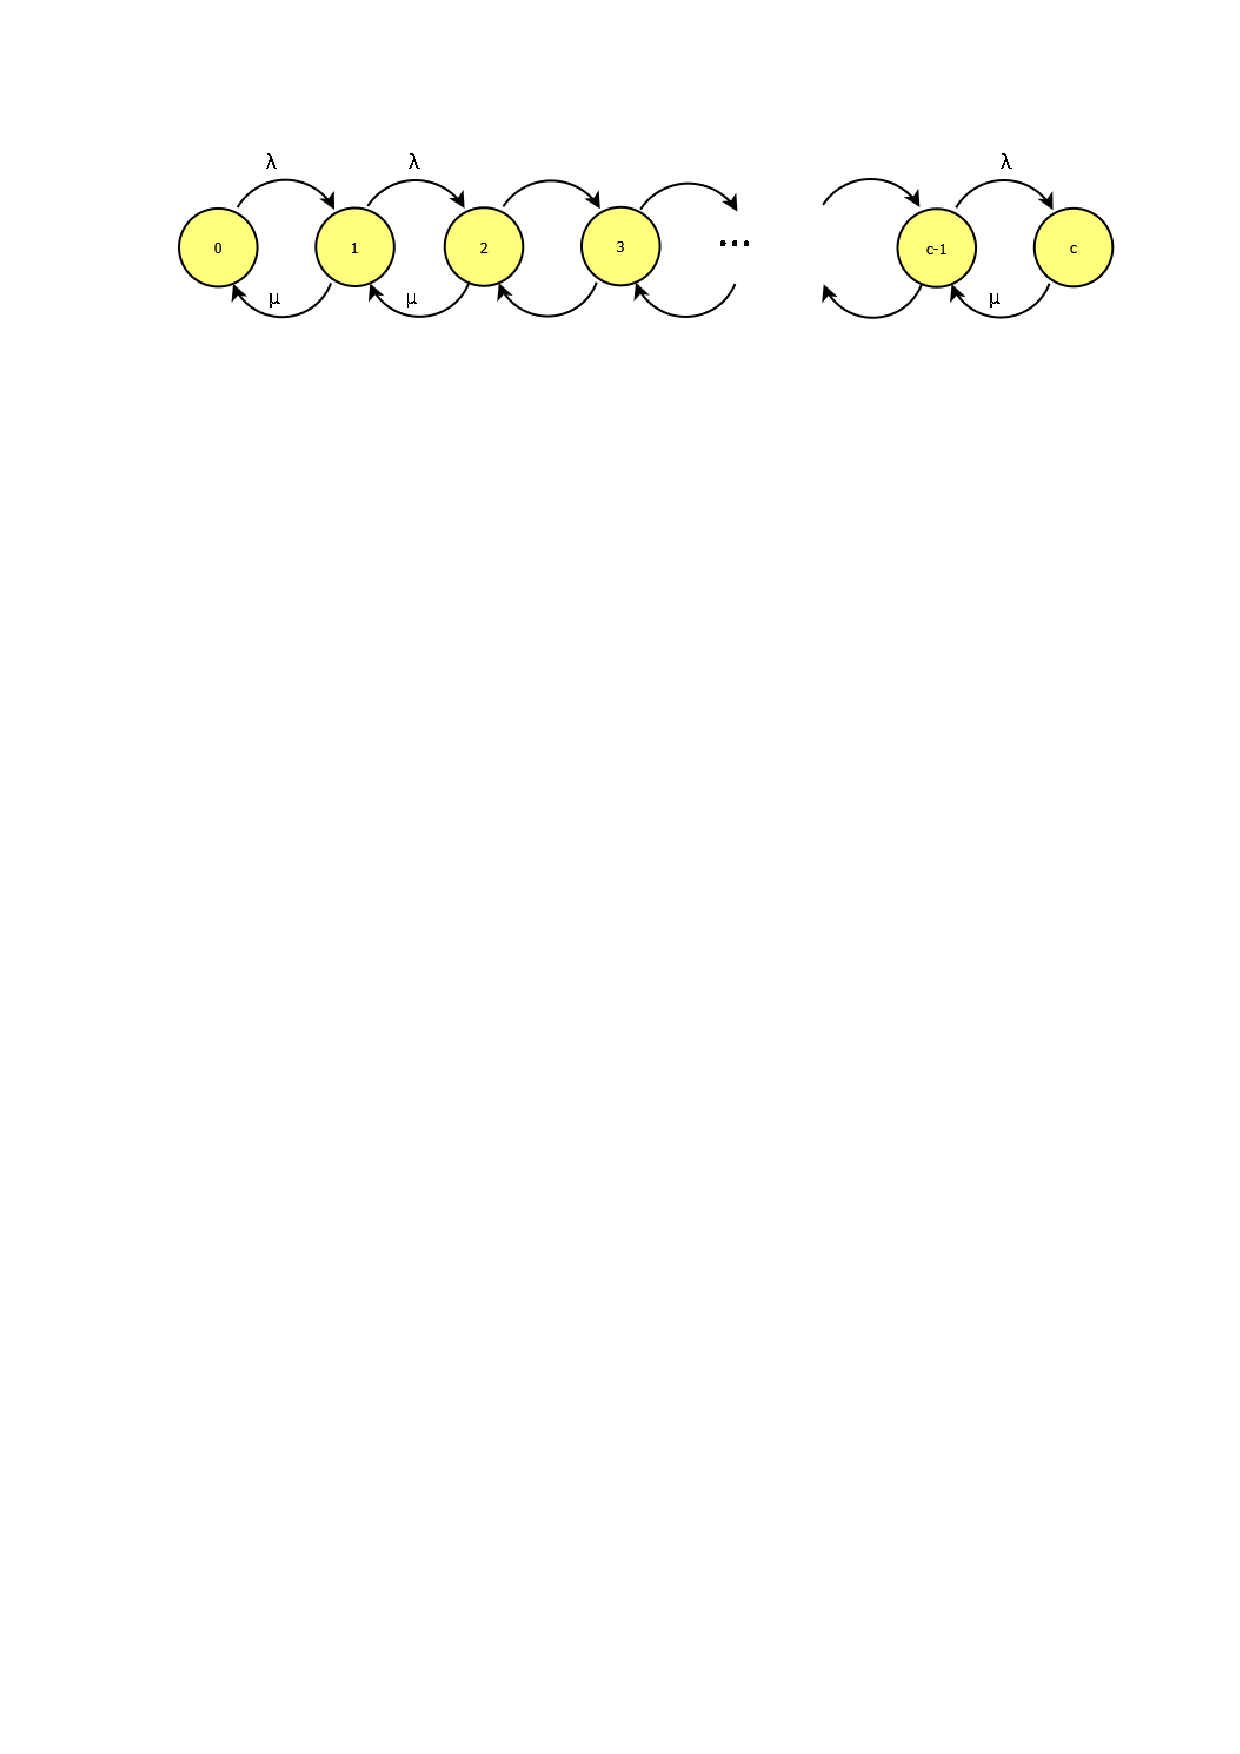
\includegraphics[trim = 10mm 220mm 10mm 25mm, clip,width=0.9\linewidth]{MMc}
		\end{figure}
		
	\section{M/M/s}
		En este modelo, la capacidad del sistema es infinita y contamos con $s$ servidores. Vamos a suponer que solo se forma una cola, y que el primero de la cola pasa al primer servidor que se quede libre. Claramente, un sistema con esta forma de espera es mucho m\'as eficiente que uno en el que se forme una cola para cada servidor, pues podr\'ia pasar que un servidor se quedase libre y nadie entrase.\\
		\hspace{0.5cm}En este modelo asumiremos que el tiempo entre llegadas es exponencial de ratio $\lambda$ y y el tiempo de servicio es exponencial de ratio $\mu$, para cada uno de los $s$ servidores.\\
		\hspace{0.5cm}Cuando en el sistema haya $j\leq s$ clientes, todos estar\'an siendo servidos. Cuando haya $j>s$, los que vayan llegando esperar\'an en la cola. Tenemos que este tipo de cola se puede modelizar como un proceso de nacimiento-muerte con los siguientes par\'ametros
		$$\begin{array}{cc}
		\lambda_j=\lambda & (j=0,1,2,...)\\
		\mu_j=j\mu & (j=1,2,...,s)\\
		\mu_j=s\mu & (j=s+1,s+2,...)\\
		\end{array}$$
		\hspace{0.5cm}Definimos $\rho=\displaystyle\frac{\lambda}{s\mu}$. Al igual que en el modelo $M/M/1$, si $\rho\geq1$, el sistema no alcanza el equilibrio pues el n\'umero de clientes se "disparar\'ia". Por lo tanto, para $\rho<1$ usando las ecuaciones de equilibrio:
		$$\begin{array}{cc}
		\pi_0=\displaystyle\frac{1}{\displaystyle \sum_{t=0}^{t=s-1}\frac{(s\rho)^t}{t!}+\frac{(s\rho)s}{s!(1-\rho)}} & \\
		\pi_j=\displaystyle\frac{(s\rho)^j\pi_0}{j!} & (j=0,1,...,s)\\
		\pi_j=\displaystyle\frac{(s\rho)^j\pi_0}{s!s^{j-s}} & (j=s+1,s+2,...)\\
		\end{array}$$
		\hspace{0.5cm} Es muy interesante saber cu\'al es la probabilidad de que todos los servidores est\'en ocupados, que viene dada por:
		$$P(j\geq s)=\sum_{k\geq s}^{}\pi_k=\sum_{k=s}^{\infty}\frac{(s\rho)^k\pi_0}{s!s^{k-s}}=\frac{s^s}{s!}\pi_0\sum_{k=s}^{\infty}\rho^k=\frac{s^s}{s!}\pi_0\rho^s\frac{1}{1-\rho}=\frac{(s\rho)^s}{s!(1-\rho)}\pi_0$$
			
		Se puede demostrar que 
		$$L_q=\frac{P(j\geq s)\rho}{1-\rho}$$
		Una vez tenemos $L_q$, usando las f\'ormulas de Little obtenemos
		$$W_q=\frac{L_q}{\lambda}=\frac{P(j\geq s)}{s\mu-\lambda}$$
		\hspace{0.5cm} Una vez que el cliente est\'a en el servidor, como este sigue una distribuci\'on exponencial, tenemos que $W_s=\frac{1}{\mu}$.\\
	    \hspace{0.5cm}	Mediante Little obtenemos $L_s=\frac{\lambda}{\mu}$. Luego
		$$L=L_q+L_s=L_q+\frac{\lambda}{\mu}$$
		De nuevo, usando Little podemos calcular $W$
		$$W=\frac{L}{\lambda}=\frac{L_q}{\lambda}+\frac{1}{\mu}$$
		
		\begin{figure}[h]
			\centering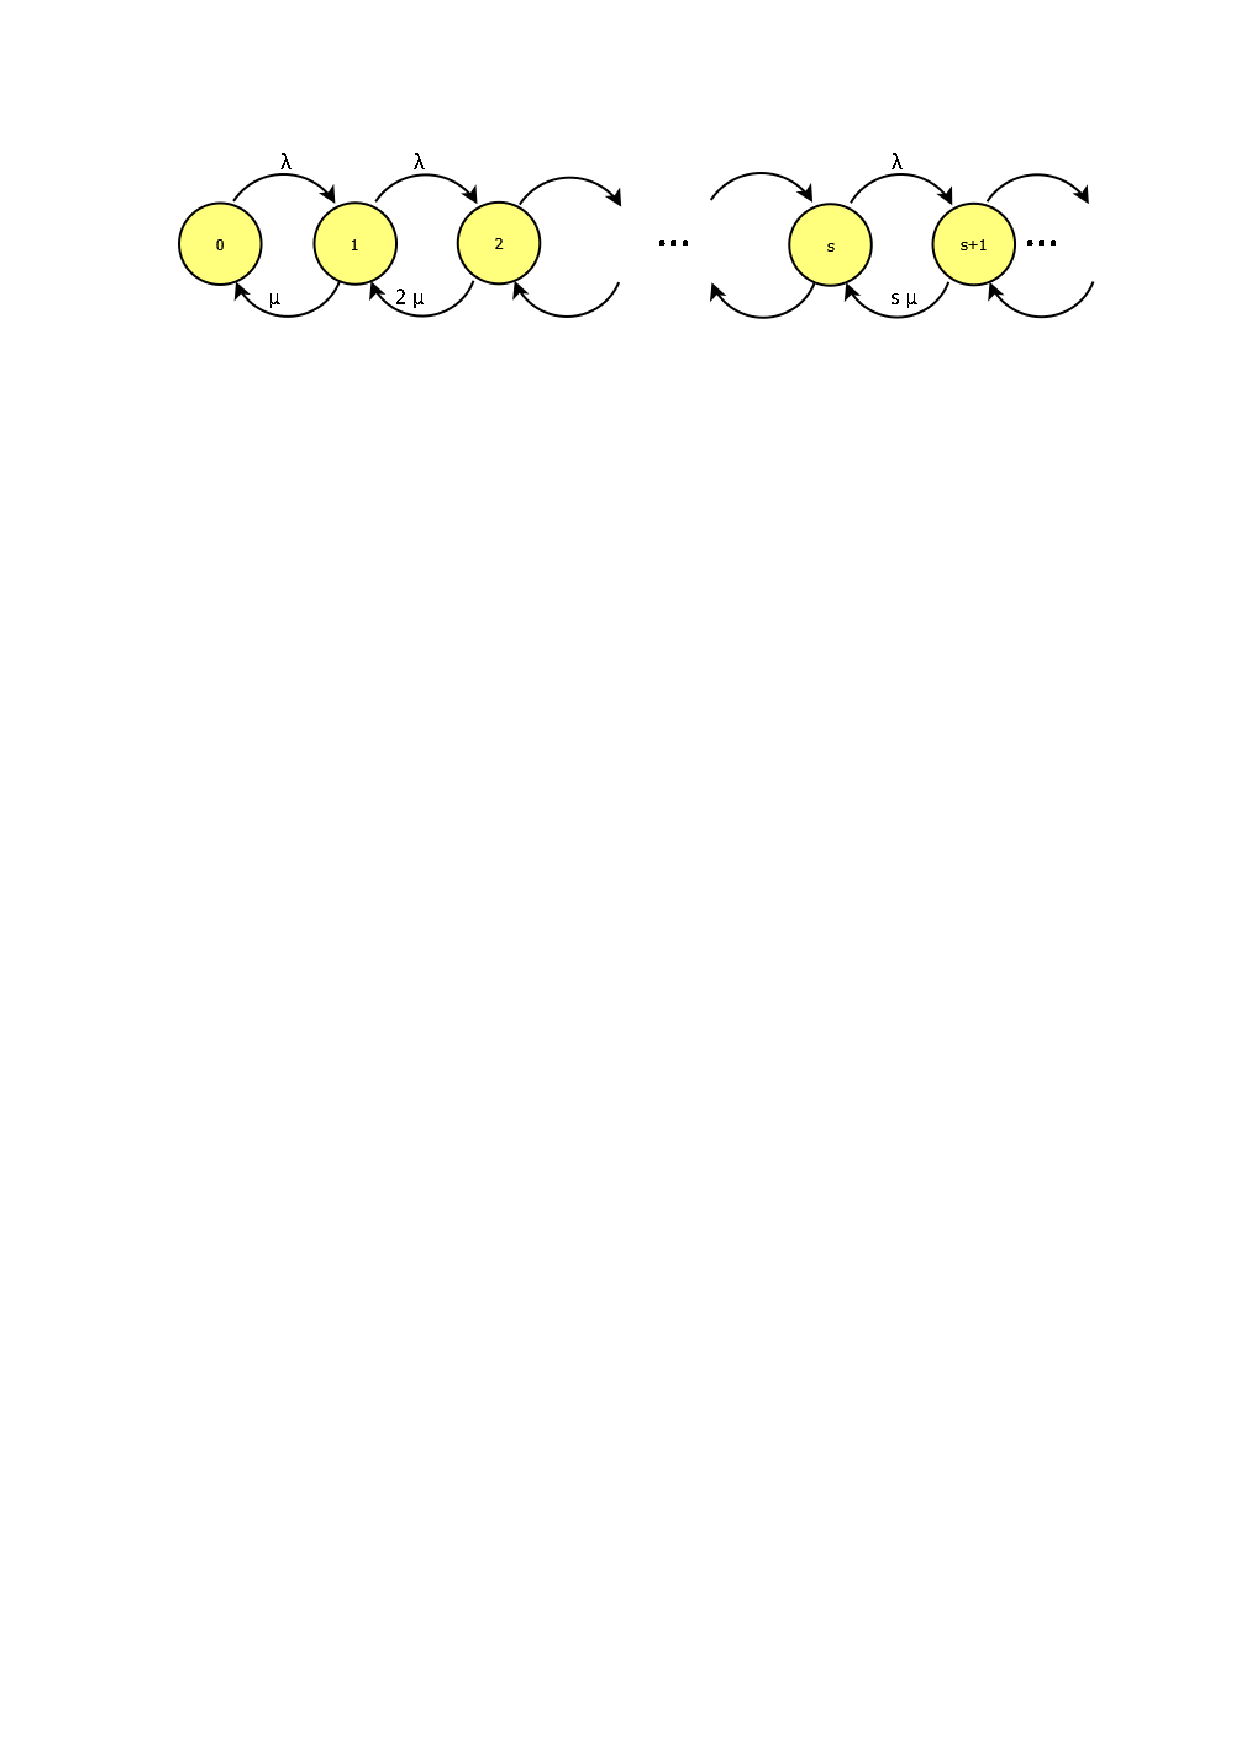
\includegraphics[trim = 10mm 220mm 10mm 25mm, clip,width=0.9\linewidth]{MMs}
		\end{figure}
		
		
		
	

% Modelos

\section{M/G/1}


Se trata de un sistema de líneas de espera con un solo servidor en el que los tiempos entre llegadas son exponenciales, pero la distribución de los tiempos de servicio no requiere ser exponencial.

Definimos

\begin{center}
$\frac{1}{\mu}=E(S)$ y   $\sigma^2= Var(S)$
\end{center}

Observamos que este modelo no es un proceso de nacimiento-muerte ya que los tiempos de servicio no tienen la propiedad de carencia de memoria de la exponencial, y la probabilidad de que el servicio se complete entre $t$ y $t + \Delta t$ cuando el estado del sistema en el tiempo $t$ es $j$ depende del tiempo transcurrido desde que se completó el último servicio.\\

Determinar las probabilidades de estado estable no es una tarea sencilla debido a que ya no son válidas las ecuaciones de estado estable en el proceso de nacimiento-muerte.

Para ello, utilizamos los resultados de Pollaczek y Khinchin para determinar $L_q$, $L$, $L_s$, $W_q$, $W$, $W_s$. Pollaczek y Khinchin demostraron que para un sistema de colas de este tipo

\begin{equation}
L_q=\frac{\lambda^2 \sigma^2+\rho}{2(1-\rho)}
\end{equation}

donde $\rho=\displaystyle\frac{\lambda}{\mu}$. Como $W_s=\displaystyle\frac{1}{\mu}$, por las fórmulas de Little se tiene que $L_s=\lambda\left(\displaystyle\frac{1}{\mu}\right)=\rho$. Como $L=L_s+L_q$ obtenemos que

\begin{equation}
L=L_q+\rho
\end{equation}

Nuevamente de las fórmulas de Little tenemos

\begin{equation}
W_q=\frac{L_q}{\lambda}\\
W=W_q+\frac{1}{\mu}
\end{equation}

		\begin{figure}[h]
			\centering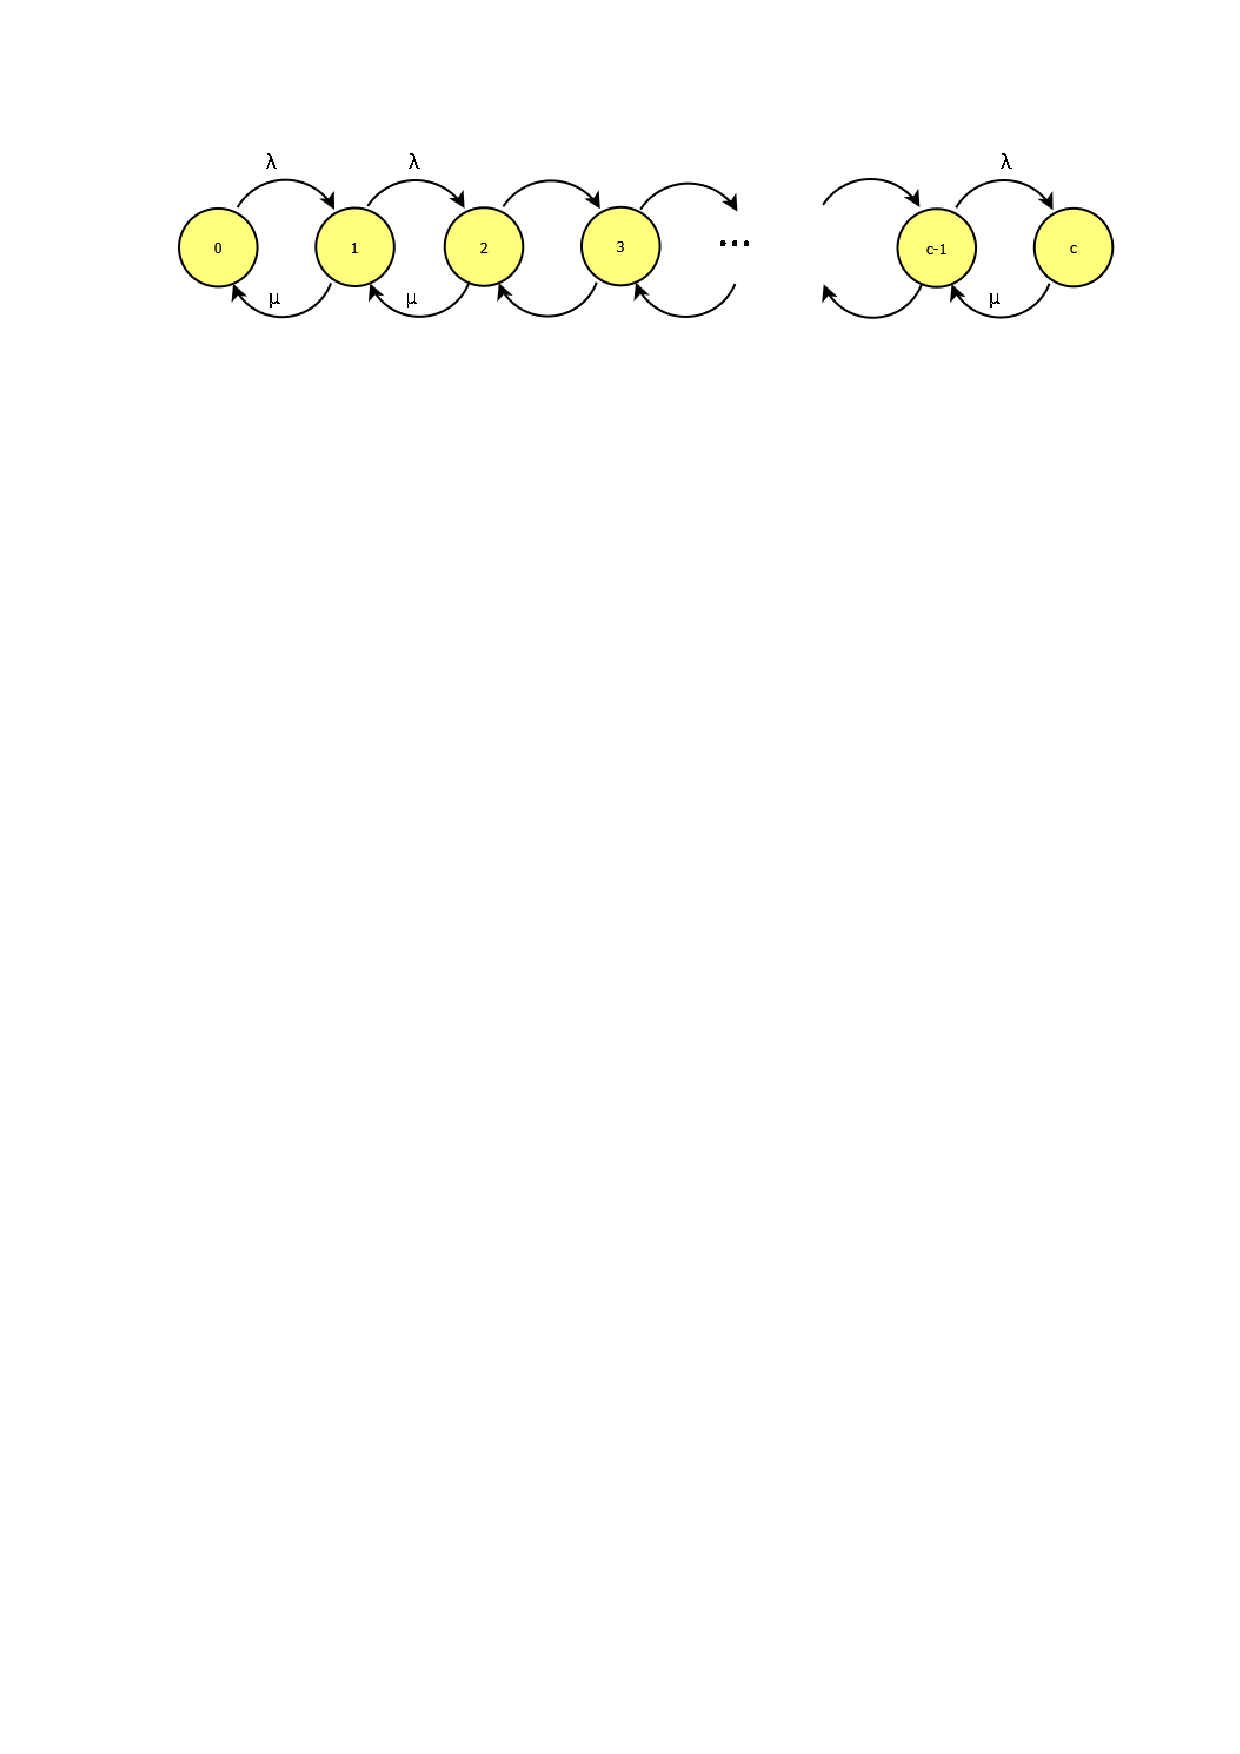
\includegraphics[trim = 10mm 220mm 10mm 25mm, clip,width=0.9\linewidth]{MMc}
		\end{figure}
		



% Anexo
\section{Anexo: Ejemplos}
\subsection{M/M/1}
Supongamos que en una estación existe un sólo servidor que llegan aproximadamente 45 clientes por hora. Se atiende a 60 clients por ahora aproximadamente. Los clientes esperan de promedio 3 minutos en la cola. \\ \\
Conocemos los siguientes datos:
$$\lambda=45 \frac{clientes}{hora}= \frac{45}{60}\frac{clientes}{minutos}$$
$$ \mu = 60 \frac{clientes}{hora} = 1 \frac{clientes}{minutos} $$
$$ W_q = 3 ~ minutos $$
\begin{enumerate}
	\item Tiempo promedio que un cliente pasa en el sistema. \\
	Para calcular el tiempo promedio que un cliente pasa en el sistema ($W_s$). Lo podemos calcular a partir de las fórmulas de esta sección, $W_1$ y $\mu$.
	$$ W_s=W_q+\frac{1}{\mu}=3+1=4 ~ minutos $$ \\
	Es decir, en promedio un cliente pasa 4 minutos en el sistema: 3 minutos apsa esperando en la cola, y un minuto en el servicio.
	\item Para calcular el número de clientes en la cola ($L_q$), usamos la fórmula de esta sección, $L_q=\lambda W_q$. 
	$$ L_q=\lambda W_q = 0.75 \frac{clientes}{minutos} 3 ~ minutos=2.25 ~ clientes$$
	Puede haber más de dos clientes en la cola.
	\item Para calcular cual es el número de clientes de la cola ($L_s$), usamos la fórmula: $L_s=\lambda W_s$.
	$$L_s=\lambda W_s = 0.75 \frac{clientes}{minutos} 4 ~ minutos=3~ clientes$$
	Es decir, en promedio hay tres en clientes en el sistema, como sabemos que sólo hay un servidor, sólo un cliente puede ser atendido. Por tanto, sólo hay dos clientes esperando.
\end{enumerate}

Un lava coches (1 servidor) es capaz de atender un coche cada 5 minutos, y la tasa media de llegadas de coches es de 9 coches por hora. Obtenga las medida de desempeño de acuerdo al modelo M/M/1. \\
Además hay que calcular la probabilidad de tener 0 clientes en el sistema, la probabildiad de tener una cola de más de 3 clientes y la probabilidad de esperar más de 30 minutos en la consola y en el sistema: \\ \\
Sabemos:
$$ \lambda = 9 \frac{clientes}{hora} = 0.15 \frac{clientes}{minutos} $$
$$ \mu = 0.2 \frac{clientes}{minutos} $$

\begin{enumerate}
	\item Primero tenemos que calcular $\rho$. \\
	$$\rho=\frac{\lambda}{\mu}=0.75=75 \%$$
	Es decir, el sistema está ocupado el $75\%$, por el complementario, el sistema está vació el $ 25 \% $ del tiempo.
	\item La probabilidad de tener más de tres clientes, las volvemos a calcular por el complementario:
	$$p^0=(1-\frac{\lambda}{\mu})(\frac{\lambda}{\mu})^0=(0.25)(0.75)^2=0.25$$
		$$p^1=(1-\frac{\lambda}{\mu})(\frac{\lambda}{\mu})^1=0.1875$$
			$$p^2=(1-\frac{\lambda}{\mu})(\frac{\lambda}{\mu})^2=0.1406$$
			$$p^3=(1-\frac{\lambda}{\mu})(\frac{\lambda}{\mu})^3=0.1055$$
	
	Esto nos da, $P(L_s \leq 3)$ pero queremos conocer $P(L_s > 3)=1-(p^0+p^1+p^2+p^3)=0.3164$
	
	\item La probablidad de esperar más 30 minutos en la cola lo hacemos del mismo modo. \\
	El tiempo que espera un cliente promedio es 
	$$ W_q=\frac{\lambda}{\mu(\mu-\lambda)}=15 ~ minutos$$
	Ahora vamos a calcular tiempo de espera sea mayor de 30 minutos. \\
	$P(W_q>t)=\rho e^{-\mu (1-\rho)t}$, a partir de aquí, calculamos la probabilidad:
	$$P(W_q > 30)=16.7\%$$
	\item Del mismo modo, para $P(W_s > t)=e^{-\mu(1-\rho)t}$:
	$$ P(W_s > 30)=22.3 \% $$
\end{enumerate} 

\subsection{M/M/s}
Actualmente una gasolinera tiene 2 bombas y está considerando agregar una tercera. Los vehículos llegan al sistema con un promedio de 1 cada 10 minutos, cada vehículo requiere de un promedio de 5 minutos para ser atendido. Supongamos que los vehículos llegan de acuerdo con una distribución Poisson y que el tiempo necesario para prestar el servicio se distribuye en forma exponencial.

$$ \frac{1}{\lambda}=\frac{1}{10} 60 \frac{min}{hora} \longrightarrow \lambda = 6 \frac{cliente}{hora} $$
$$ \frac{1}{\mu} = \frac{1}{5} 60  \frac{min}{hora} \longrightarrow \mu = 12 \frac{clientes}{hora} $$
\begin{enumerate}
	\item Determine la razón de utlización del sistema \\ \\ $\rho=\frac{\lambda}{s \mu}=\frac{6}{2 \cdot 12}=25 \%$, esto es el tiempo que se está utilizando, es decir, el sistema está vacío el $75 \%$ del tiempo.
\end{enumerate}

\subsection{M/M/1/c}
El promedio de llegada de coches a una joyería es de 20 coches por hora. El servicio es capaz de procesar 8 coches por hora. El único aparcamiento de la joyería está restringido a 6 coches. El porcentaje de llegada sigue una distribución de Poisson. Analizar que pasaría si el servicio fuese capaz de procesar 20 coches por hora. \\ \\
Sabemos:
$$\lambda=20 \frac{coches}{horas} $$
$$ \mu = 18 \frac{coches}{horas} $$ 

$$ N = 6 ~ coches $$
Y también sabemos que el promedio es de $\rho=1.11$, por tanto podemos calcular los siguientes valores:
$$P_{N=6}=\left[\frac{1-\rho}{1-\rho^{N+1}}p^N\right]=0.1917$$
$$L_s=\rho \left[\frac{1-(N+1)\rho + N \rho ^{N+1}}{(1-\rho)(1-\rho^{N+1})}\right]=3.41 ~ coches$$
$$\lambda_e= \lambda(1-P_N)=16.166$$
$$L_q=L_s-(1-P_0)$$
$$P_0=0.1019$$
$$L_q=2.512 ~ coches $$
$$ W_q=W_s-\frac{1}{\mu}=1.1553 ~ horas$$
Por otro lado, si el servicio pasase a poder procesar 20 coches por horas, entonces:
$$\mu=\lambda$$
$$\rho=1$$
Entonces, $L_s$ puede escribirse de la siguiente forma:
$$L_s=\frac{N}{2}=\frac{6}{2}=3~ coches$$
\newpage

\section{Anexo: Software}
% http://www.supositorio.com/rcalc/rcalclite.htm

A continuación, exponemos una herramienta que sirve para calcular los valores de la teoría de cola para cada modelo.
\begin{figure*}[h]
	\centering
	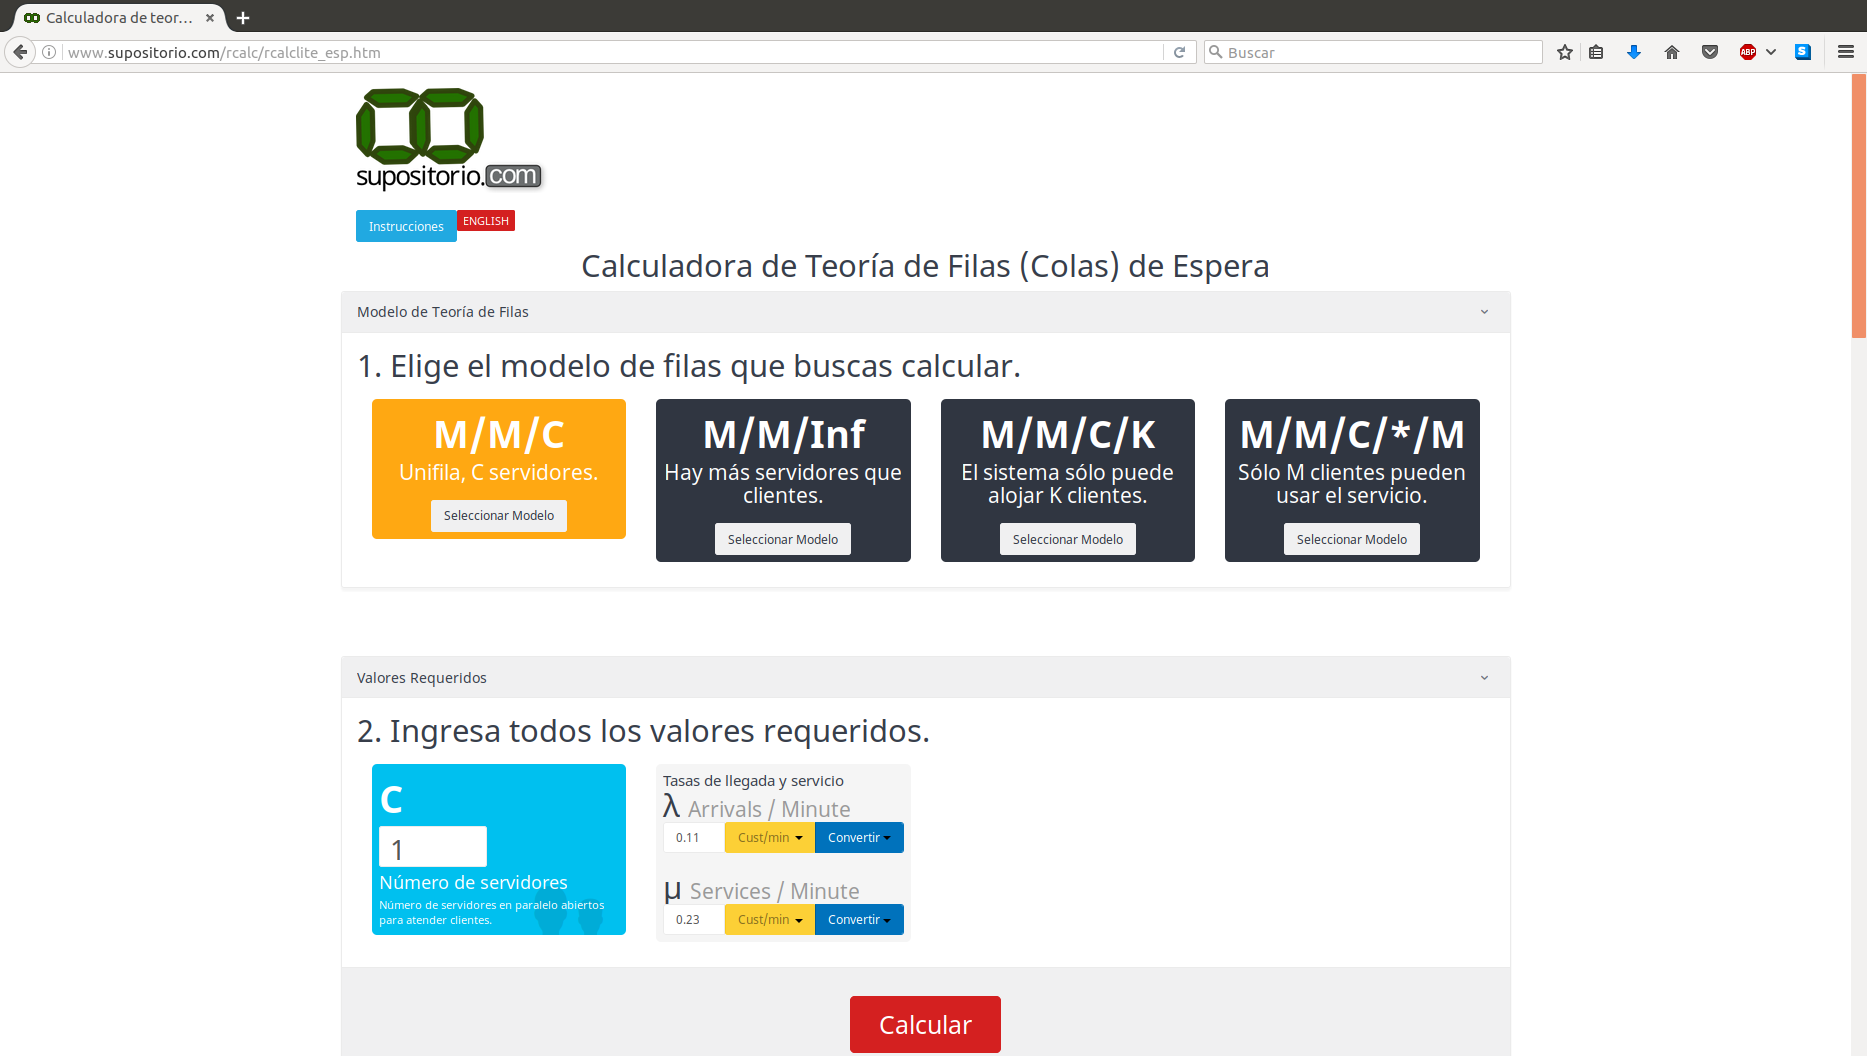
\includegraphics[width=0.6\textwidth]{soft1}
	\label{soft1}
	\caption{Pantalla principal}
\end{figure*}
\newpage
En la pantalla principal de esta página web tenemos una pantalla donde se nos muestran los módelos principales de la teoría de cola. \\
A continuación, por cada modelo, nos pide los parámetros necesarios para calcular las probabilidades de cada modelo, y además, nos muestra gráficas y nos permite calcular probabilidades fácilmente.

\begin{figure*}[h]
	\centering
	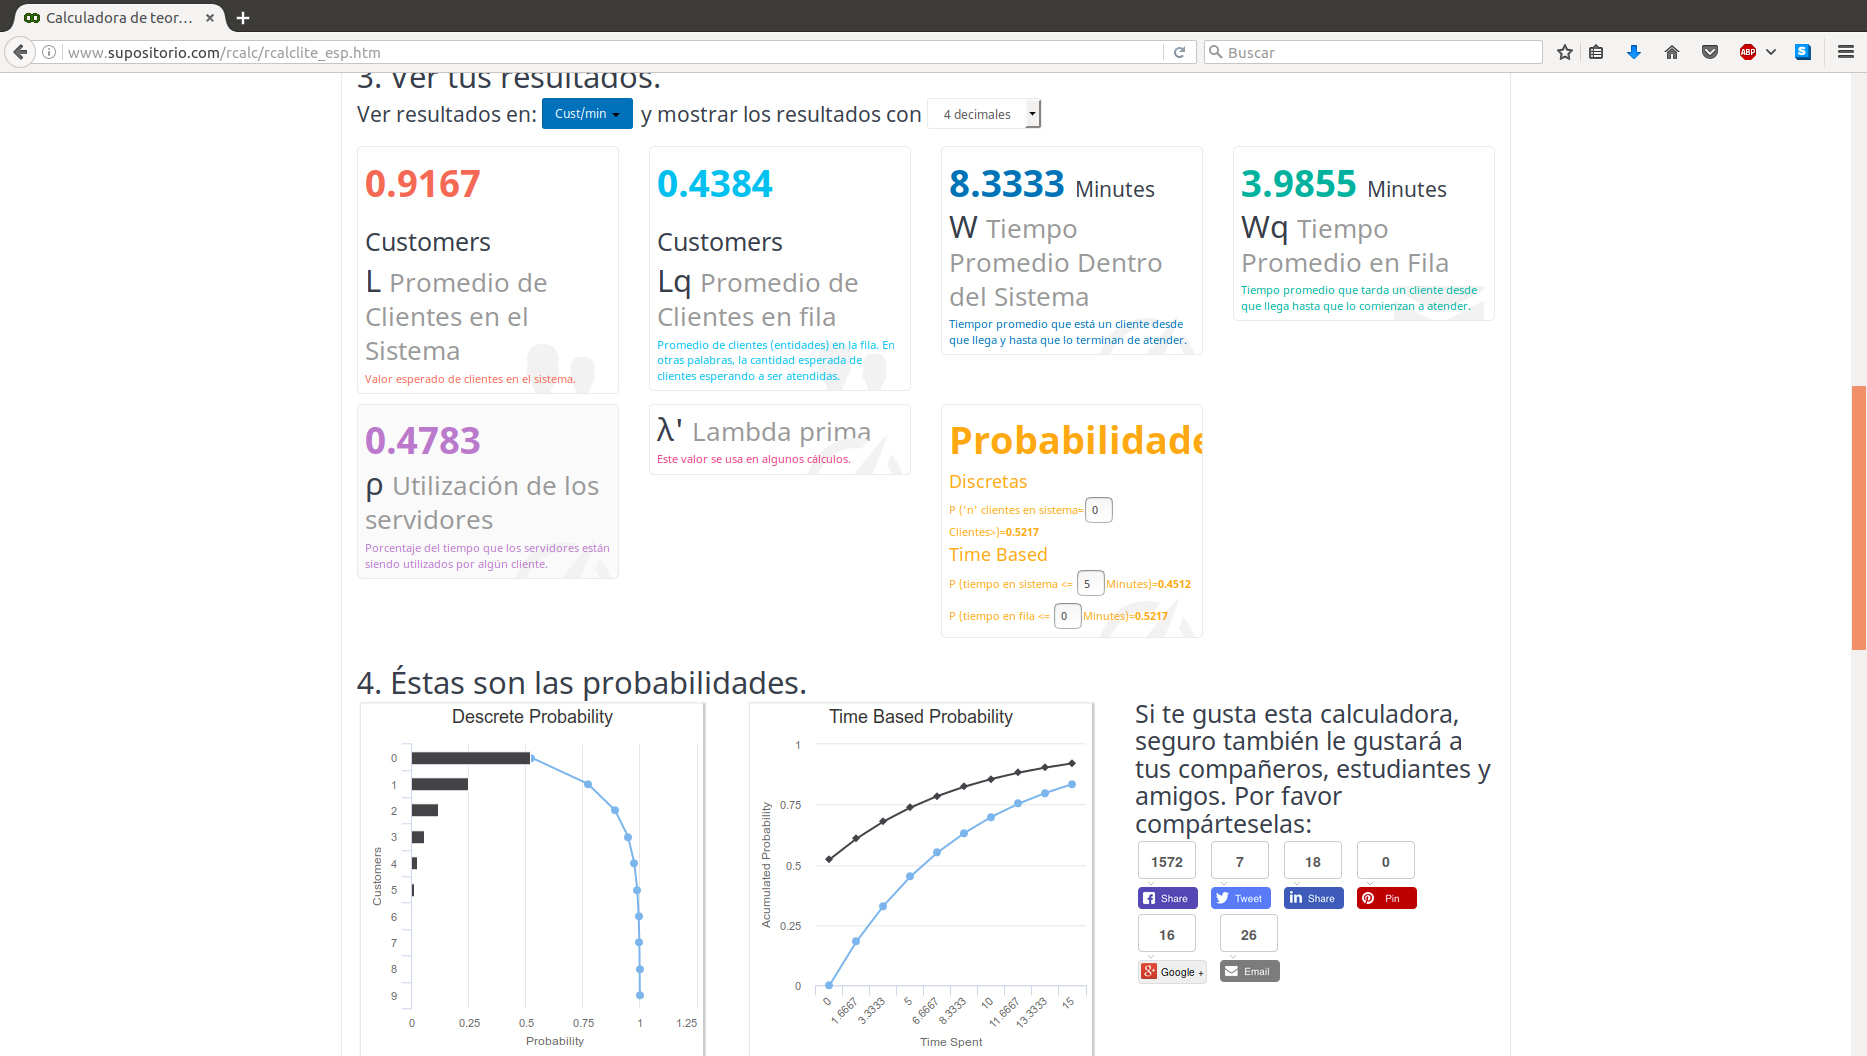
\includegraphics[width=\textwidth]{soft2}
	\label{soft2}
	\caption{Output}
\end{figure*}

Para acceder a este sitio hay que entrar a \href{http://www.supositorio.com/rcalc/rcalclite_esp.htm}{este enlace}, o si lo prefieres escribe en tu navegador: http://goo.gl/DKq59l

% Autores
\section{Referencia}
\begin{enumerate}
	\item Investigación de operaciones - Wayne L. Winston.
	\item Applied Stochastics Processes - Mario Lefebvre
	\item Apuntes del curso 'Procesos estocásticos y series temporales' - Miguel Ángel Sordo Díaz
\end{enumerate}

\section{Autores}
\begin{itemize}
	\item José Carlos García Ortega
	\item Álvaro Ramírez Moreno
	\item Juan Manuel Pérez Sánchez
	\item Marina Gandullo Escobar
\end{itemize}


% Licencia
\section{Código fuente}
Este documento está protegido con la licencia GPL3 y puedes descargar una copia de la licencia y el código fuente de este PDF en el siguiente enlace:
\begin{itemize}
	\item \href{https://github.com/JoseCarlosGarcia95/mio-tex}{https://github.com/JoseCarlosGarcia95/mio-tex}
\end{itemize}
\begin{center}
    \href{http://creativecommons.org/licenses/by-sa/3.0/es/}{\includegraphics[width=4em]{cc-by-sa}}
\end{center}
\end{document}
